

\begin{frame}{MERX como representaci\'on intermedia}
    \begin{columns}[T]
        \begin{column}{0.48\linewidth}
            \vspace{25mm}

            \resizebox{\linewidth}{!}{
            \begin{tikzpicture}
                \tikzstyle{every entity} = [minimum width=2.3cm, minimum height=1.2cm]
                \node[entity] (jugador) at (0,0) {JUGADOR};
                \node[entity] (carta) at (9,0) {CARTA};
                \node[relationship, aspect=2] (coleccionar) at (4.5,0) {COLECCIONAR} edge(jugador) edge(carta);
                \node at (7.5,0.2) {$1,\ast$};
                \node at (1.5,0.2) {$0,\ast$};
            \end{tikzpicture}
            }
        \end{column}

        \begin{column}{0.48\linewidth}
            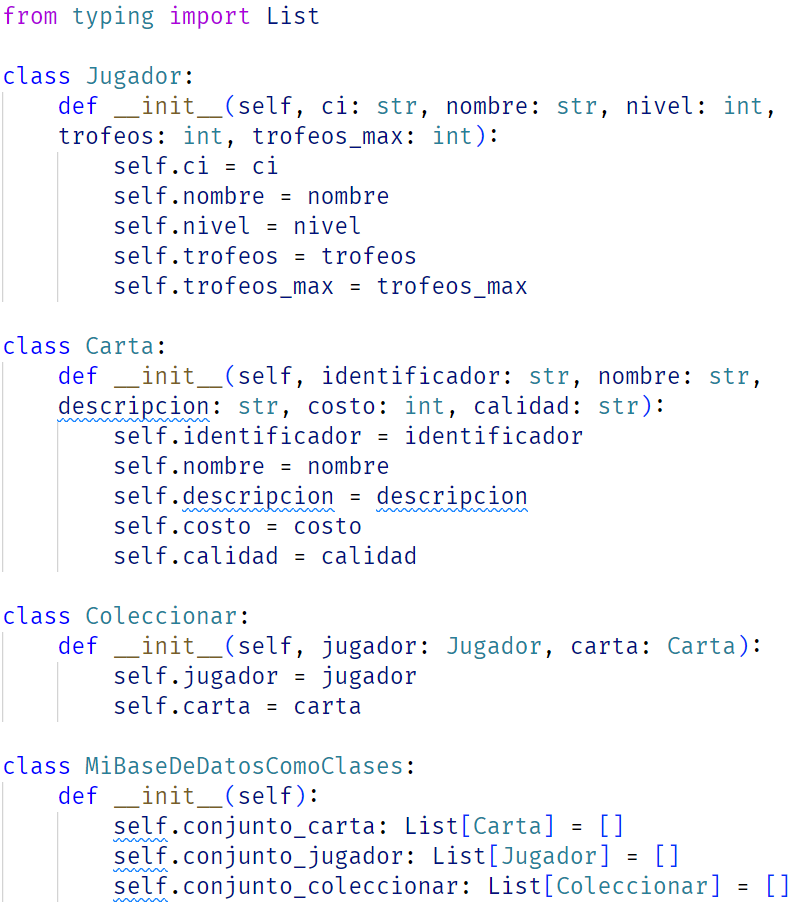
\includegraphics[width=0.9\linewidth, height=0.75\textheight]{img/classes.png}
        \end{column}
        
    \end{columns}
\end{frame}

\begin{frame}{MERX como representaci\'on intermedia}
    \begin{columns}[T]
        \begin{column}{0.48\linewidth}
            \vspace{25mm}

            \resizebox{\linewidth}{!}{
            \begin{tikzpicture}
                \tikzstyle{every entity} = [minimum width=2.3cm, minimum height=1.2cm]
                \node[entity] (jugador) at (0,0) {JUGADOR};
                \node[entity] (carta) at (9,0) {CARTA};
                \node[relationship, aspect=2] (coleccionar) at (4.5,0) {COLECCIONAR} edge(jugador) edge(carta);
                \node at (7.5,0.2) {$1,\ast$};
                \node at (1.5,0.2) {$0,\ast$};
            \end{tikzpicture}
            }
        \end{column}


        \begin{column}{0.48\linewidth}
            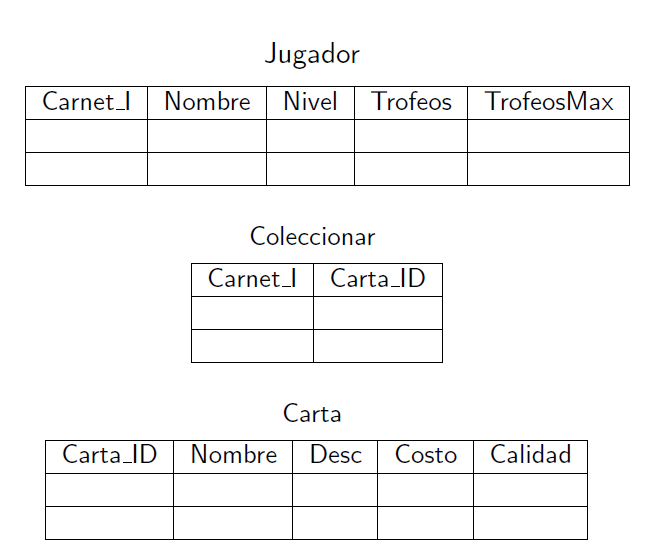
\includegraphics[width=\linewidth, height=0.75\textheight]{img/tables.png}
            % \centering
            % Jugador
            % \vspace{2mm}

            % \small
            % \begin{tabular}{|c|c|c|c|c|}
            %     \hline
            %     Carnet\_I & Nombre & Nivel & Trofeos & TrofeosMax\\
            %     \hline
            %     & & & &\\
            %     \hline
            %     & & & & \\
            %     \hline
            % \end{tabular}

            % \vspace{5mm}
            
            % \centering
            % Coleccionar
            % \vspace{2mm}
            
            % \begin{tabular}{|c|c|}
            %     \hline
            %     Carnet\_I & Carta\_ID \\
            %     \hline
            %     & \\
            %     \hline
            %     & \\
            %     \hline
            % \end{tabular}
            
            % \vspace{5mm}

            % \centering
            % Carta
            % \vspace{2mm}

            % \begin{tabular}{|c|c|c|c|c|}
            %     \hline
            %     Carta\_ID & Nombre & Desc & Costo & Calidad\\
            %     \hline
            %     & & & & \\
            %     \hline
            %     & & & & \\
            %     \hline
            % \end{tabular}
        \end{column}
        
    \end{columns}
\end{frame}